\hrefsection{tsfi.ls.wan}{\tsfisectionname{ls.wan}}

\lswan{} is a logical interface to the IT products in the WAN. It is 
accessible via the physical interface \intf{PS.WAN}. The interface comprises the
protocols listed in \tableref{tab:ls.lwan.protocols-ports} together with their
port numbers. \figureref{fig:tsfi.ls.lwan.protocols} depicts the protocols that
contribute to the security aspects of the TSFI (see also the introductory
remarks in \chapterref{tsfi.ls}.


\afterpage{%
  \clearpage% Flush earlier floats (otherwise order might not be correct)
  \begin{landscape}% Landscape page
    \centering % Center table
    {
      \label{tab:ls.wan.protocols-ports}
      \begin{longtable}{@{}lcllcclp{6cm}@{}}
        \toprule
        Service & In/Out & Protocol & via & Source port & Dest. port & TSFI & Note \\ \midrule \endhead
        \bottomrule \caption*{Protocols und port numbers for IP/TCP/UDP on \formatintf{LS.WAN}} \endfoot
        \bottomrule \caption{Protocols und port numbers for IP/TCP/UDP on \formatintf{LS.WAN}} \endlastfoot
        Base protocols & -- & IEEE802.3 &  -- & -- & -- &    \tsfilink{ls.wan.ether} \\
                & -- & IPv4 & IEEE802.3 & -- & -- &    \tsfilink{ls.wan.ip} \\
                & -- & TCP &  IPv4 & -- & -- &    \tsfilink{ls.wan.tcp} \\
                & -- & UDP &  IPv4 & -- & -- &    \tsfilink{ls.wan.udp} \\[2ex]
        IPSec & Out & IKEv2 & UDP & dyn. & 500 & \tsfilink{ls.wan.ipsec} \\
                & Out & IKEv2 & UDP & dyn. & 4500 & \tsfilink{ls.wan.ipsec} & for UDP-Encapsulation\\
                & -- & ESP & IPv4 & -- & -- &   \tsfilink{ls.wan.ipsec} \\
                & -- & ESP & UDP & dyn. &  4500 & \tsfilink{ls.wan.ipsec} & for UDP-Encapsulation\\[2ex]
        Zeitdienst   & Out & NTP  & UDP & -- & 123 &    \tsfilink{ls.wan.ntp} \\[2ex]
        DHCP-Service & Out & DHCP & UDP & 68 & 67 &    \tsfilink{ls.wan.dhcp} \\[2ex]
      \end{longtable}
    }
  \end{landscape}
  \clearpage% Flush page
}

\begin{figure}[htbp]
  \centering
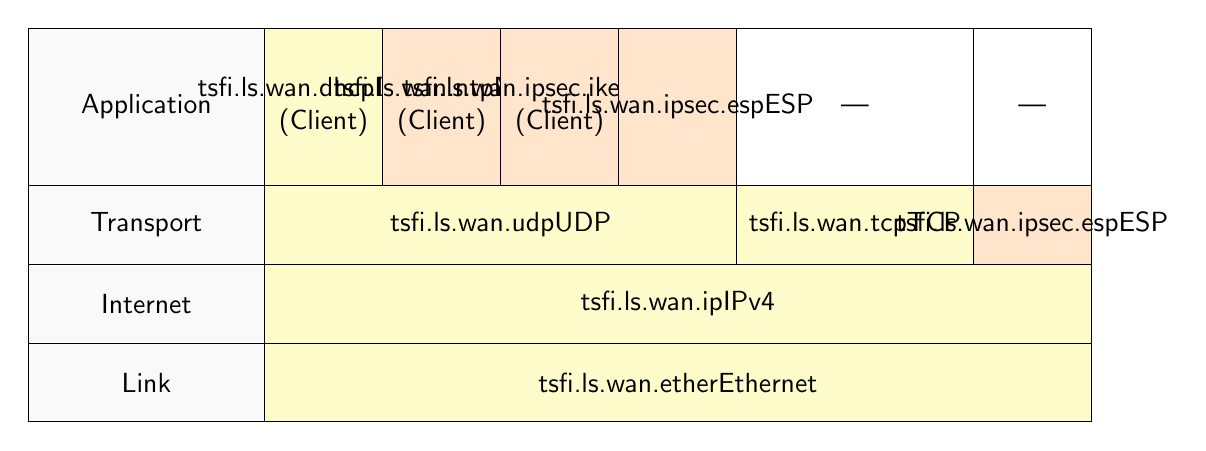
\begin{tikzpicture}
    [c/.style={midway,align=center,font=\sffamily},
      tsfi/.style={fill=orange!20},
      nontsfi/.style={fill=yellow!20},
      none/.style={},      
      layer/.style={fill=gray!5}]

  \draw[layer] (0,0) rectangle ++(3,1) node[c]{Link};
  \draw[nontsfi] (3,0) rectangle ++(10.5,1) node[c]{\hyperlink{tsfi.ls.wan.ether}{Ethernet}};

  \draw[layer] (0,1) rectangle ++(3,1) node[c]{Internet};
  \draw[nontsfi] (3,1) rectangle ++(10.5,1) node[c]{\hyperlink{tsfi.ls.wan.ip}{IPv4}};

  \draw[layer] (0,2) rectangle ++(3,1) node[c]{Transport};
  \draw[nontsfi] (3,2) rectangle ++(6,1) node[c]{\hyperlink{tsfi.ls.wan.udp}{UDP}};
  \draw[nontsfi] (9,2) rectangle ++(3,1) node[c]{\hyperlink{tsfi.ls.wan.tcp}{TCP}};
  \draw[tsfi] (12,2) rectangle ++(1.5,1) node[c]{\hyperlink{tsfi.ls.wan.ipsec.esp}{ESP}};

  \draw[layer] (0,3) rectangle ++(3,2) node[c]{Application};
  \draw[nontsfi] (3,3) rectangle ++(1.5,2) node[c]{\hyperlink{tsfi.ls.wan.dhcp}{DHCP} \\ (Client)};
  \draw[tsfi] (4.5,3) rectangle ++(1.5,2) node[c]{\hyperlink{tsfi.ls.wan.ntp}{NTP} \\ (Client)};
  \draw[tsfi] (6,3) rectangle ++(1.5,2) node[c]{\hyperlink{tsfi.ls.wan.ipsec.ikev2}{IKEv2} \\ (Client)};
  \draw[tsfi] (7.5,3) rectangle ++(1.5,2) node[c]{\hyperlink{tsfi.ls.wan.ipsec.esp}{ESP}};
  \draw[none] (9,3) rectangle ++(3,2) node[c]{---};
  \draw[none] (12,3) rectangle ++(1.5,2) node[c]{---};

\end{tikzpicture}
  \caption{Protocols on \formatintf{LS.WAN} for the TSFI}
  \label{fig:tsfi.ls.wan.protocols}
\end{figure}


\hrefsubsection{tsfi.ls.wan.ether}{\tsfisectionname{ls.wan.ether}}

\sameprotocol{Ethernet}{WAN}{tsfi.ls.lan.ether}

\hrefsubsection{tsfi.ls.wan.ip}{\tsfisectionname{ls.wan.ip}}

\sameprotocol{IPv4 und ICMP}{WAN}{tsfi.ls.lan.ip}

\hrefsubsection{tsfi.ls.wan.tcp}{\tsfisectionname{ls.wan.tcp}}

\sameprotocol{TCP}{WAN}{tsfi.ls.lan.tcp}

\hrefsubsection{tsfi.ls.wan.udp}{\tsfisectionname{ls.wan.udp}}

\sameprotocol{UDP}{WAN}{tsfi.ls.lan.udp}

\hrefsubsection{tsfi.ls.wan.dhcp}{\tsfisectionname{ls.wan.dhcp}}

\tsfipurpose{tsfi.ls.wan.dhcp}

The TOE provides the capability to act as an DHCP client on the WAN
interface. The TOE obtain its IP address from a DHCP server in the WAN. This function can be activated/deactivated with the management interface \lslanhttpmgmt{}.

\calledenforcingsfr{ls.wan.dhcp}

\calledsupportingsfr{ls.wan.dhcp}

\calledsfmanual{ls.wan.dhcp}{\secfunclink{sf.networkservices}}

\tsfiparameters{tsfi.ls.wan.dhcp}

DHCP is implemented according to \rfc[c]{2131}.

\tsfiactions{tsfi.ls.wan.dhcp}

\tsfierrormessages{tsfi.ls.wan.dhcp}

\hrefsubsection{tsfi.ls.wan.ntp}{\tsfisectionname{ls.wan.ntp}}

\tsfipurpose{tsfi.ls.wan.ntp}

This interface is used to synchronize the system time with time servers in the
WAN.

\calledenforcingsfr{ls.wan.ntp}

\calledsupportingsfr{ls.wan.ntp}

\calledsf{ls.wan.ntp}

\tsfiparameters{tsfi.ls.wan.ntp}

The protocol is specified in \rfc[c]{5905} dokumentiert. The destination port
for the client is UDP port~123.

\tsfiactions{tsfi.ls.wan.ntp}

\tsfierrormessages{tsfi.ls.wan.ntp}


\hrefsubsection{tsfi.ls.wan.ipsec}{\tsfisectionname{ls.wan.ipsec}}

\tsfipurpose{tsfi.ls.wan.ipsec}

The TOE uses the WAN interface to establish the VPN channel with IPsec.

\calledenforcingsfr{ls.wan.ipsec}

\calledsupportingsfr{ls.wan.ipsec}

\calledsf{ls.wan.ipsec}

\tsfiparameters{tsfi.ls.wan.ipsec}

The TOE fulfills the requirements from \rfc[c]{4301}. It uses two protocols for
IPsec. Key exchange is implemented by IKE version 2 according to
\rfc[c]{7296}. User data is tranmitted via the Encapsulation Security Payload
(ESP) according to\rfc[c]{4303}. 

\tsfiactions{tsfi.ls.wan.ipsec}

\tsfierrormessages{tsfi.ls.wan.ipsec}


\hrefsubsubsection{tsfi.ls.wan.ipsec.ikev2}{Internet Key Exchange Version 2 (IKEv2)}

IKE is used for the distribution of key material and the authentication of the
peers. The TOE is initiator of VPN connections and thus submits the suitable algorithms.


\hrefsubsubsection{tsfi.ls.wan.ipsec.esp}{Encrypted Security Payload (ESP)}

ESP provides authenticity, integrity and confidentiality for the transmitted
data. Separate algorithms for encryption and integrity protection are used. The
negotiated SA including the required keys and algorithm are used to secure the
and IP packets sent over the tunnel. ESP headers have the structure shown in
\figureref{fig:tsfi.ls.wan.ipsec.esp.header} (see also
\cite[Figure~2]{rfc4303}).


\begin{figure}[htbp]
  \centering
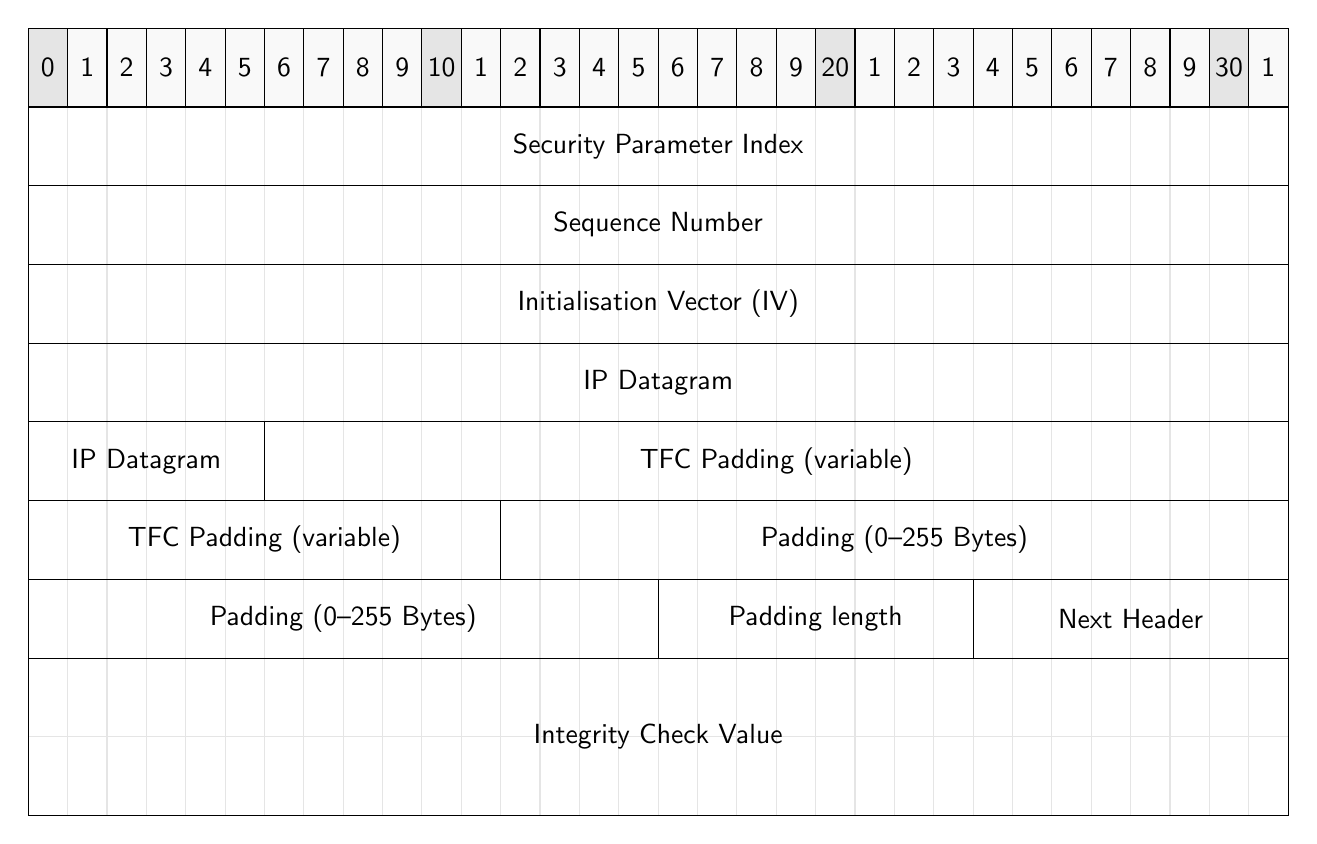
\begin{tikzpicture}
  [c/.style={midway,font=\sffamily},
  none/.style={},
  index/.style={fill=gray!5},
  index0/.style={fill=gray!20}]

  \draw[xstep=.5,gray!20, thin] (0,0) grid (16,9);

  \draw[index] (15.5,9) rectangle ++(0.5,1) node[c]{1};
  \draw[index0] (15,9) rectangle ++(0.5,1) node[c]{30};
  \draw[index] (14.5,9) rectangle ++(0.5,1) node[c]{9};
  \draw[index] (14,9) rectangle ++(0.5,1) node[c]{8};
  \draw[index] (13.5,9) rectangle ++(0.5,1) node[c]{7};
  \draw[index] (13,9) rectangle ++(0.5,1) node[c]{6};
  \draw[index] (12.5,9) rectangle ++(0.5,1) node[c]{5};
  \draw[index] (12,9) rectangle ++(0.5,1) node[c]{4};
  \draw[index] (11.5,9) rectangle ++(0.5,1) node[c]{3};
  \draw[index] (11,9) rectangle ++(0.5,1) node[c]{2};
  \draw[index] (10.5,9) rectangle ++(0.5,1) node[c]{1};
  \draw[index0] (10,9) rectangle ++(0.5,1) node[c]{20};
  \draw[index] (9.5,9) rectangle ++(0.5,1) node[c]{9};
  \draw[index] (9,9) rectangle ++(0.5,1) node[c]{8};
  \draw[index] (8.5,9) rectangle ++(0.5,1) node[c]{7};
  \draw[index] (8,9) rectangle ++(0.5,1) node[c]{6};
  \draw[index] (7.5,9) rectangle ++(0.5,1) node[c]{5};
  \draw[index] (7,9) rectangle ++(0.5,1) node[c]{4};
  \draw[index] (6.5,9) rectangle ++(0.5,1) node[c]{3};
  \draw[index] (6,9) rectangle ++(0.5,1) node[c]{2};
  \draw[index] (5.5,9) rectangle ++(0.5,1) node[c]{1};
  \draw[index0] (5,9) rectangle ++(0.5,1) node[c]{10};
  \draw[index] (4.5,9) rectangle ++(0.5,1) node[c]{9};
  \draw[index] (4,9) rectangle ++(0.5,1) node[c]{8};
  \draw[index] (3.5,9) rectangle ++(0.5,1) node[c]{7};
  \draw[index] (3,9) rectangle ++(0.5,1) node[c]{6};
  \draw[index] (2.5,9) rectangle ++(0.5,1) node[c]{5};
  \draw[index] (2,9) rectangle ++(0.5,1) node[c]{4};
  \draw[index] (1.5,9) rectangle ++(0.5,1) node[c]{3};
  \draw[index] (1,9) rectangle ++(0.5,1) node[c]{2};
  \draw[index] (0.5,9) rectangle ++(0.5,1) node[c]{1};
  \draw[index0] (0,9) rectangle ++(0.5,1) node[c]{0};

  \draw[none] (0,8) rectangle ++(16,1) node[c]{Security Parameter Index};

  \draw[none] (0,7) rectangle ++(16,1) node[c]{Sequence Number};

  \draw[none] (0,6) rectangle ++(16,1) node[c]{Initialisation Vector (IV)};

  \draw[none] (0,5) rectangle ++(16,1) node[c]{IP Datagram};

  \draw[none] (3,4) rectangle ++(13,1) node[c]{TFC Padding (variable)};
  \draw[none] (0,4) rectangle ++(3,1) node[c]{IP Datagram};

  \draw[none] (6,3) rectangle ++(10,1) node[c]{Padding~(0--255 Bytes)};
  \draw[none] (0,3) rectangle ++(6,1) node[c]{TFC Padding (variable)};

  \draw[none] (12,2) rectangle ++(4,1) node[c]{Next Header};
  \draw[none] (8,2) rectangle ++(4,1) node[c]{Padding length};
  \draw[none] (0,2) rectangle ++(8,1) node[c]{Padding~(0--255 Bytes)};

  \draw[none] (0,0) rectangle ++(16,2) node[c]{Integrity Check Value};

\end{tikzpicture}
  \caption{ESP Header}
  \label{fig:tsfi.ls.wan.ipsec.esp.header}
\end{figure}



% !TEX root = "../adv_fsp"
%%% Local Variables:
%%% mode: latex
%%% TeX-engine: luatex
%%% TeX-master: "../adv_fsp"
%%% TeX-parse-self: t
%%% TeX-auto-save: t
%%% End:
